\subsection*{Træning} \label{sec:traening}
Når brugeren har angivet sin daglige helbredstilstand samt, hvilken træningsform, der ønskes kan træningen begyndes. Aktivitetsdiagrammet over træningen fremgår af \autoref{fig:traening}. 

\begin{figure} [H]
\centering
\textbf{Aktivitetsdiagram: Træning}\par\medskip
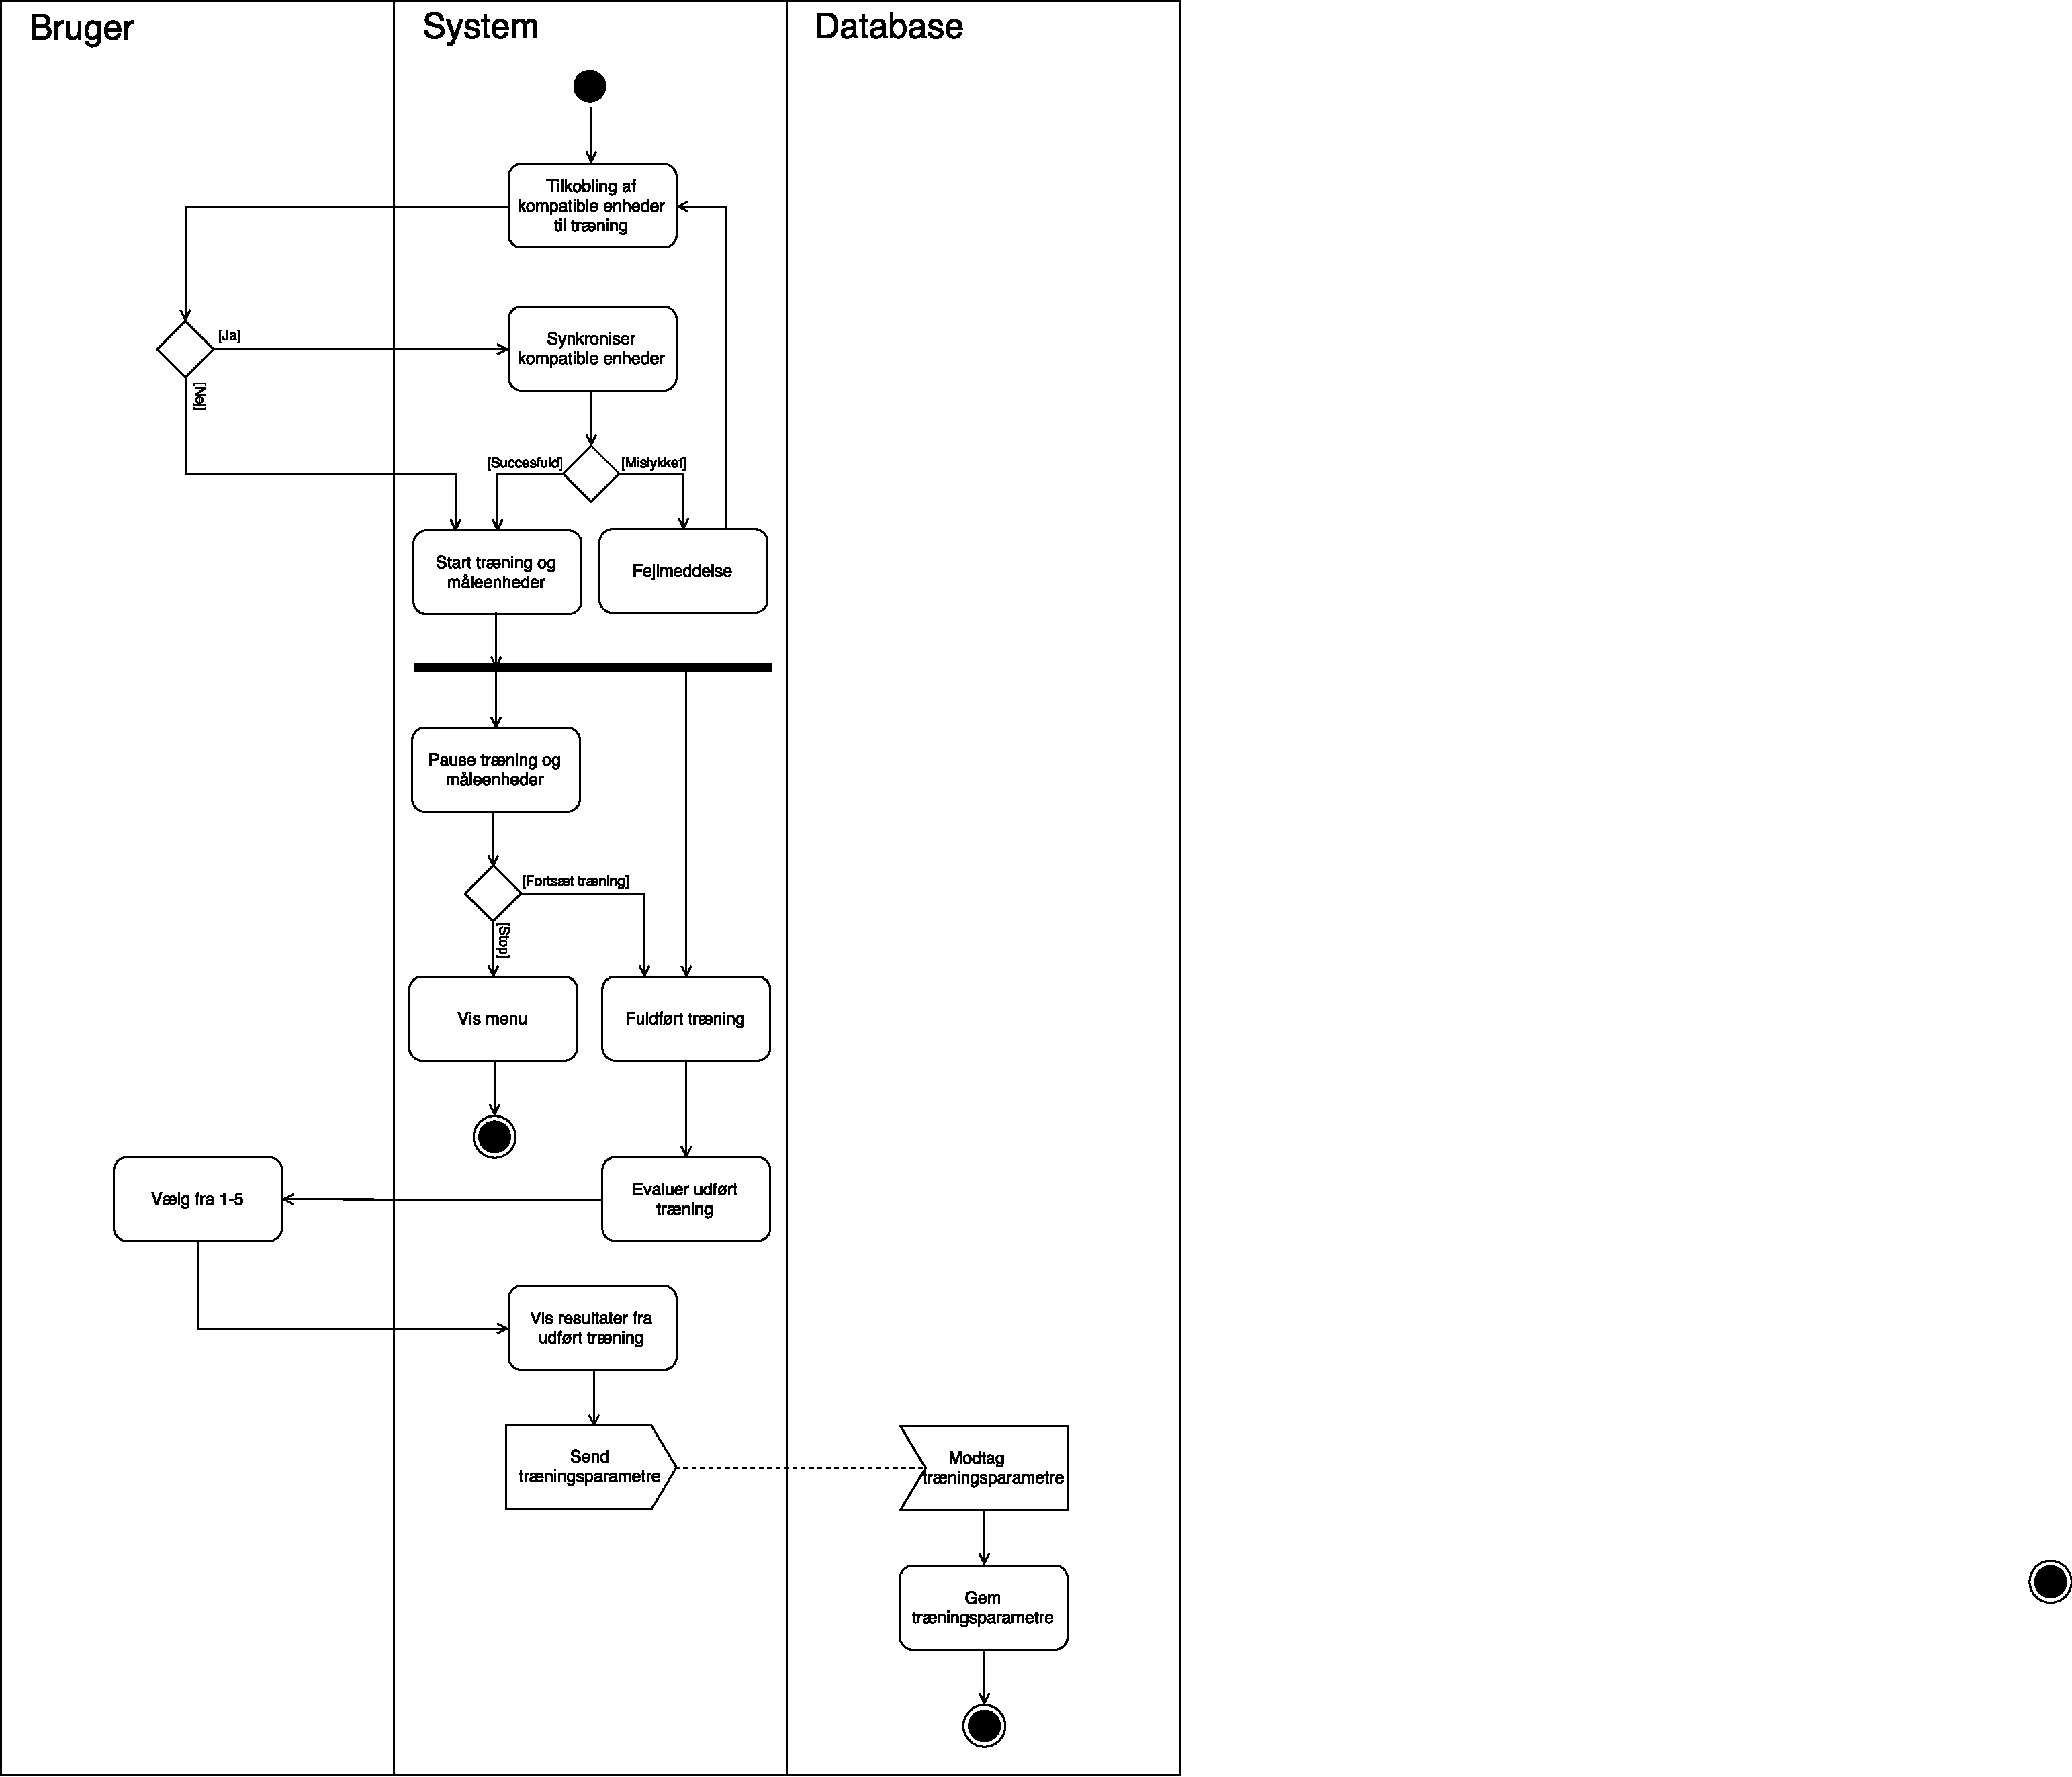
\includegraphics[width=0.9\textwidth]{figures/aktivitetsdiagram/Traening}
\caption{Aktivitetsdiagram over træning.}
\label{fig:traening}
\end{figure}

\noindent
Før selve træningen kan påbegyndes, kan der tilkobles kompatible enheder til systemet, eksempelvis pulsmåler. Vælger brugeren ikke at tilkoble eksterne enheder, startes timer og GPS, hvorefter selve træningen påbegyndes. Vælger brugeren derimod at tilkoble enheder, prøver systemet at synkronisere med enhederne.  Hvis dette lykkes, påbegyndes selve træningen og alle måleenhederne starter. Lykkes dette ikke, sender systemet en fejlmeddelelse, og brugeren skal igen angive om de vil tilkoble enheder til systemet.

Under træningen kan brugeren pause træningen og måleenhederne, hvorefter der er mulighed for at fortsætte træningen eller afslutte træningen. Afsluttes eller fuldføres træningen, skal brugere evaluere træningen. Denne evalueres som let, moderat eller hård. Herefter vises resultater fra den udførte træning. Systemet sender træningsparametre, som består af den daglige helbredstilstand, resultater fra den udførte træning samt evaluering til databasen, som lagrer informationerne. 